%% Fall 2013 MDM Homework Template
\documentclass[12pt,letterpaper]{article}

\usepackage[utf8]{inputenc}
\usepackage[T1]{fontenc}
\usepackage{amsmath}
\usepackage{amsfonts}
\usepackage{amssymb}
\usepackage[left=2cm,right=2cm,top=2cm,bottom=2cm,headheight=22pt]{geometry}
\usepackage{fancyhdr}
\usepackage{setspace}
\usepackage{lastpage}
\usepackage{graphicx,subcaption}

\usepackage{amsthm}

\theoremstyle{definition}
\newtheorem{task}{Task}

\begin{document}

%other parameters
\setlength{\parskip}{1ex plus 0.5ex minus 0.2ex}
\setlength{\parindent}{0pt}

%header and footer parameters
\pagestyle{fancy}
\lhead{Math 1100 sections 02 \& 04}
\chead{Weekly Homework}
\rhead{Due: Friday, February 19, 2016}
\lfoot{}
\cfoot{\emph{Prof. Hitchman}}
\rfoot{}

\begin{center}
{
\Large
\textbf{Written Assignment \# 5}
}
\end{center}

Your paper should have the following information on it.
\begin{itemize}
\item Your name
\item Your student ID number 
\item Which section you are in: 02 MWF, or 04 TTh
\end{itemize}


\subsection*{Specifications for Grading}

To earn a passing mark, your assignment must:
\begin{itemize}
\item be typed, and no more than three pages in length. Diagrams may be hand drawn.
\item address the writing prompts below.
\item conform to reasonable standards for grammar, spelling, and usage of the English language with minimal errors. (You may consider seeking help on writing from the Writing Center in the Academic Learning Center. http://www.uni.edu/unialc/writing-center)
\item be turned in by 3pm on Friday, February 17.
\end{itemize}


All of the tasks below have to do with a single set-up: a weird game of chance I just invented. Here is how it works:

There are two players, call them Player A and Player B. Player A has two ten-sided dice. Player B has a single twenty-sided die. Have you seen these before? Here is a picture:

\begin{figure}[h]
\centering
\begin{subfigure}[b]{0.3\textwidth}
\centering
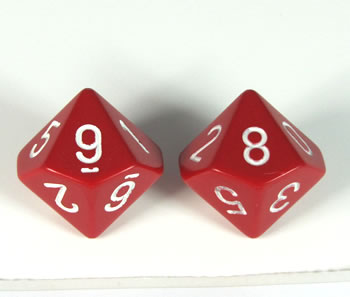
\includegraphics[width=\textwidth]{images/d10pair.jpg}
\caption{A pair of ten-sided dice}
\end{subfigure}
\quad
\begin{subfigure}[b]{0.3\textwidth}
\centering
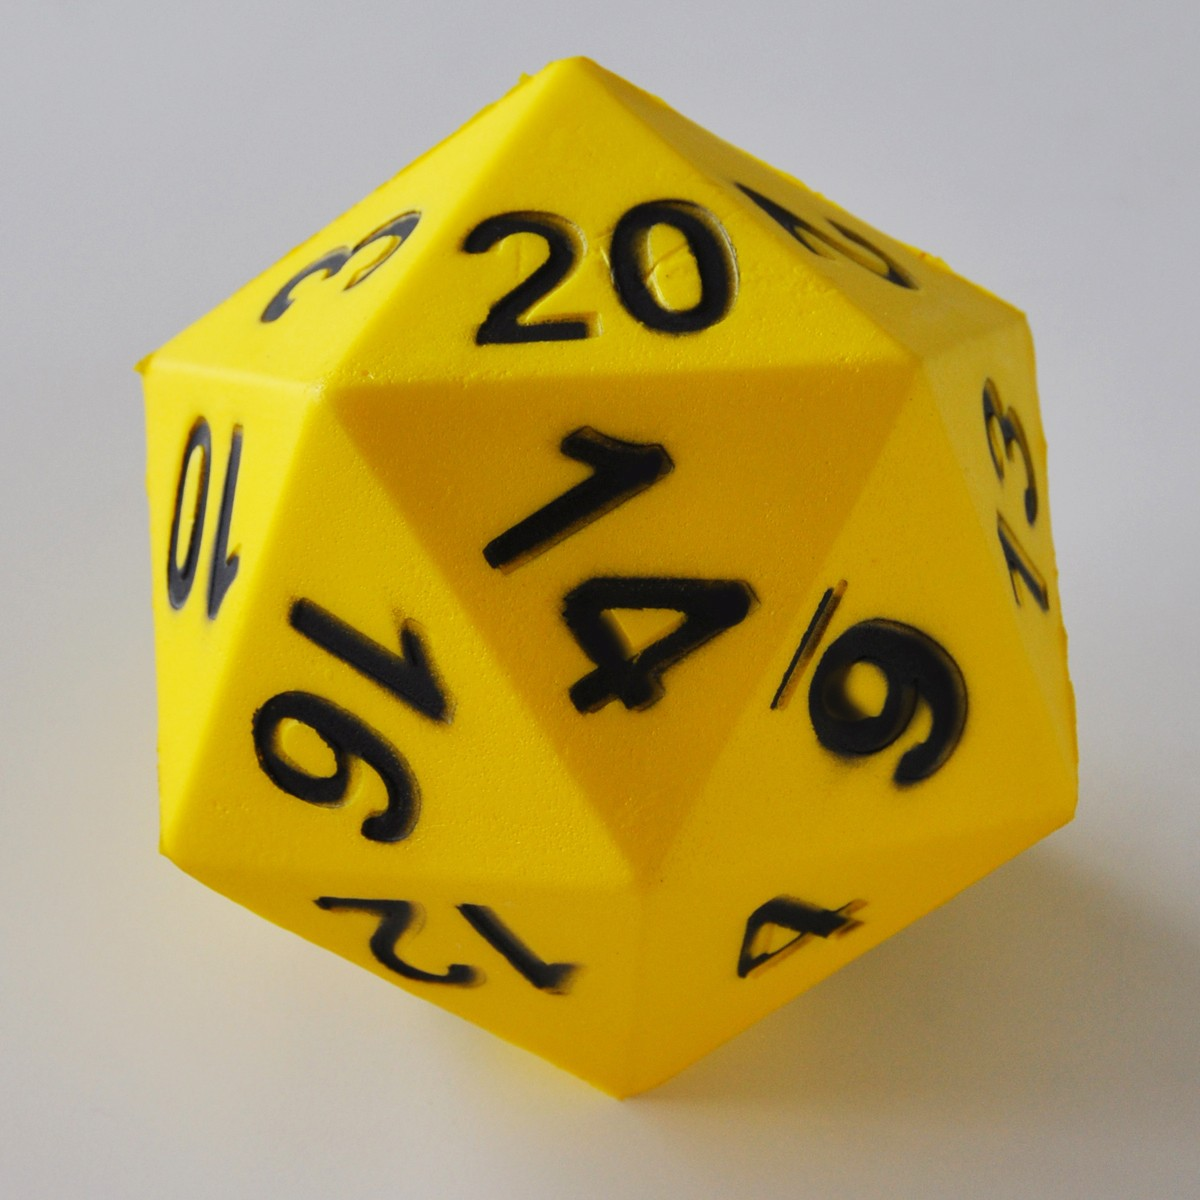
\includegraphics[width=\textwidth]{images/d20.jpg}
\caption{A twenty-sided die}
\end{subfigure}
\caption{Dice for this assignment}
\end{figure}

They behave a lot like the usual six-sided kind, except that there are more sides. The ten-sided dice are labeled with numbers 0, 1, 2, 3, 4, 5, 6, 7, 8, 9. The twenty-sided die is labeled with the numbers 1 through 20. The players roll the dice and compare numbers. Player A gets to add the two numbers she rolled. Player B just has to keep the one number he rolls.

\begin{task}
We can think about a single run of this game as a ``trial'' of a chance situation. Here the trial involves rolling three dice. Make a decision tree which will help you think about this game. 
\end{task}

\begin{task}
Use the decision tree to figure out what is the probability that Player A scores an ``11'' and Player B scores a `5'.
Explain how the decision tree helps you.
\end{task}

\begin{task}
Analyze this game carefully, and decide which player has an advantage, if either. Explain how you know your answer is the correct one.
\end{task}



\end{document}
%sagemathcloud={"zoom_width":100}